%Describe the computational experiments you conducted to validate the approach you took.
%Describe the NW Architecture
%What activations and why
%how was it optimized
%conducted on all 5 years

\begin{table*}[htb]
  \begin{center}
    \caption{Comparison of AUC score obtained using each technique}  
    \begin{tabular}{| >{\centering\arraybackslash}m{1.6in} || *5{>{\centering\arraybackslash}m{0.4in}|} @{}m{0pt}@{}}
    \hline
    \textbf{Year} & 1 & 2 & 3 & 4 & 5 &\\[2ex] 
    \hline
    \hline
    \textbf{Net2Net} & 0.967 & 0.944 &0.927 & 0.930 & 0.959 &\\[0ex]
    \hline
    \textbf{FCN} & 0.959 & 0.899 &0.903 & 0.899 & 0.945 &\\[0ex]
    \hline
    \textbf{FCN\footnote[1]{123}} & 0.543 & 0.514 &0.548 & 0.596 & 0.699 &\\[0ex]
    \hline
    \textbf{Ensemble Boosted Trees\footnote[1]{123}} & 0.959 & 0.944 &0.940 & 0.941 & 0.955 &\\[0ex]
    \hline
  \end{tabular}
  \label{tab:compare}
  \end{center}
\end{table*}
%\footnote{Footnote fdvva}
\footnotetext[1]{\cite{zikeba2016ensemble}}



\section{Metric of Performance}
\label{sec:metric}
As we discussed in section \ref{sec:proposed_method} all of the five dataset are skewed with almost $97\%$ of the majority class and rest being the other. So, in such a case, making Accuracy (that is checking $\%$ correct) as the Metric of Performance is not the right approach. The reason behind this is that the algorithm can end up predicting always the majority class and still achieve accuracy as \texttildelow$97\%$. Due to this problem we decide to use Area under the ROC curves (AUC\_ROC score) as the Metric of Performance. 

%\textbf{F1 Score:} In statistical analysis of binary classification, the F1 score (also F-score or F-measure) is a measure of a test's accuracy. It considers both the precision p and the recall r of the test to compute the score: p is the number of correct positive results divided by the number of all positive results, and r is the number of correct positive results divided by the number of positive results that should have been returned. The F1 score can be interpreted as a weighted average of the precision and recall, where an F1 score reaches its best value at 1 and worst at 0 \cite{F1}.

%\begin{align}
%  \begin{aligned}   
%  F1 = 2  \bigg( \frac{1}{\frac{1}{recall} + \frac{1}{precision}} \bigg)
%    \\
%    F1 = 2  \bigg( \frac{precision.recall}{precision + recall} \bigg)
%    \end{aligned}
% \end{align}

\textbf{Area Under the ROC Curve (AUC\_ROC):} A Receiver Operating Characteristic (ROC) curve is the most commonly used way to visualize the performance of a binary classifier \cite{dataSchool}. In statistics, a receiver operating characteristic curve, or ROC curve, is a graphical plot that illustrates the performance of a binary classifier system as its discrimination threshold is varied. The curve is created by plotting the true positive rate (TPR) against the false positive rate (FPR) at various threshold settings \cite{ROC}. Figure~\ref{fig:ROC} shows the ROC curve for year1 data of the dataset. The area under the ROC curve equals the probability that a randomly chosen positive example ranks above (is deemed to have a higher probability of being positive than) a randomly chosen negative example.

\begin{figure}[!htb]
\centering
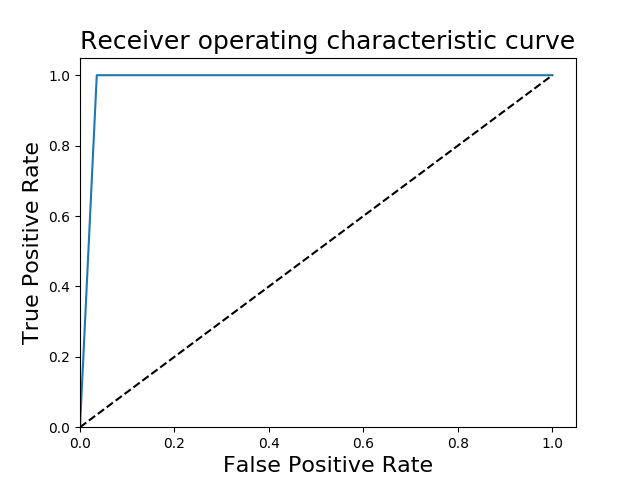
\includegraphics[width=80mm]{ROC.png}
\caption{Receiver Operating Characteristic Curve for year 1 data with the AUC score of 0.9670}
\label{fig:ROC}
\end{figure}

\section{Experiment}

\subsection{Wellness Analysis of SMOTE Data}
To confirm if the classes in the generated dataset (by SMOTE) are distributed similar to the original dataset, we implement a basic anomaly detection algorithm using Auto-Encoder with Neural Networks. For this test, we normalize all the features of the safe class and the bankrupt class separately. Then, we train the Auto-Encoder using $80\%$ safe company data of the original dataset. Then for the remaining original dataset ($20\%$ of the safe class and all of the bankrupt class) we check the reconstruction error of the dataset. Based on this error we distinguish it as safe or bankrupt. The algorithm can classify with AUC score of 0.995. Next we pass all of the generated data (SMOTE data) through the Auto-Encoder (trained on original data) and classify based on the reconstruction error. The algorithm classifies the generated data with an AUC score of 0.998. So, we confirm that both the original and generated dataset have similar distribution. We do not use this algorithm as our one of our results because we normalize the safe company data and bankrupt company data separately, thus having a prior knowledge of the data classification, to train the Auto-Encoder algorithm. 

\subsection{Model Training}

We first implement a Network model using the Net2Net technique. The technique used for training all the Net2Net networks utilized the following hyper parameters. All the models were trained with Adam as the optimizer and binary\_crossentropy was used as the cost metric to train the network. PReLu were used as the activation units as better results were obtained with this over ReLu, sigmoid and tanh. The learning rate was scheduled with initial value being the default $5\mathrm{e}{-3}$ (for Adam optimizer) and a reduction in learning rate by a factor of 10 was effected whenever the loss failed to reduce in 3 consecutive epochs. Training was performed for 2000 Epochs for each teacher network. Scaling of the network was done by widening the network first and then deepening it. Widening operation was done to a maximum of 128 neurons and then deepening operations were performed up to 8 hidden layers (discussed in detail in section \ref{sec:results}). We implemented our network models using the software package Keras \cite{chollet2015keras}. For year1 data, we start to train the network with 1 neuron and scale it to 8 hidden layers with 128 neurons in each layer. For the subsequent years, we use some of the knowledge gained in training network for year1. While training for year2, 3, 4 and 5 we chop off the network at layer4 and add layers 5, 6, 7 and 8. The intuition behind choosing to chop off at layer 4 is discussed in Section~\ref{sec:discuss}

After developing an optimized model using the Net2Net technique, we train the same network architecture using conventional method. We compare the results of the two techniques in section \ref{sec:results}. 

